\documentclass{standalone}
\usepackage{tikz}
\usetikzlibrary{patterns, positioning}
\usepackage[sfdefault]{ClearSans} %% option 'sfdefault' activates Clear Sans as the default text font
\usepackage[T1]{fontenc}

\begin{document}
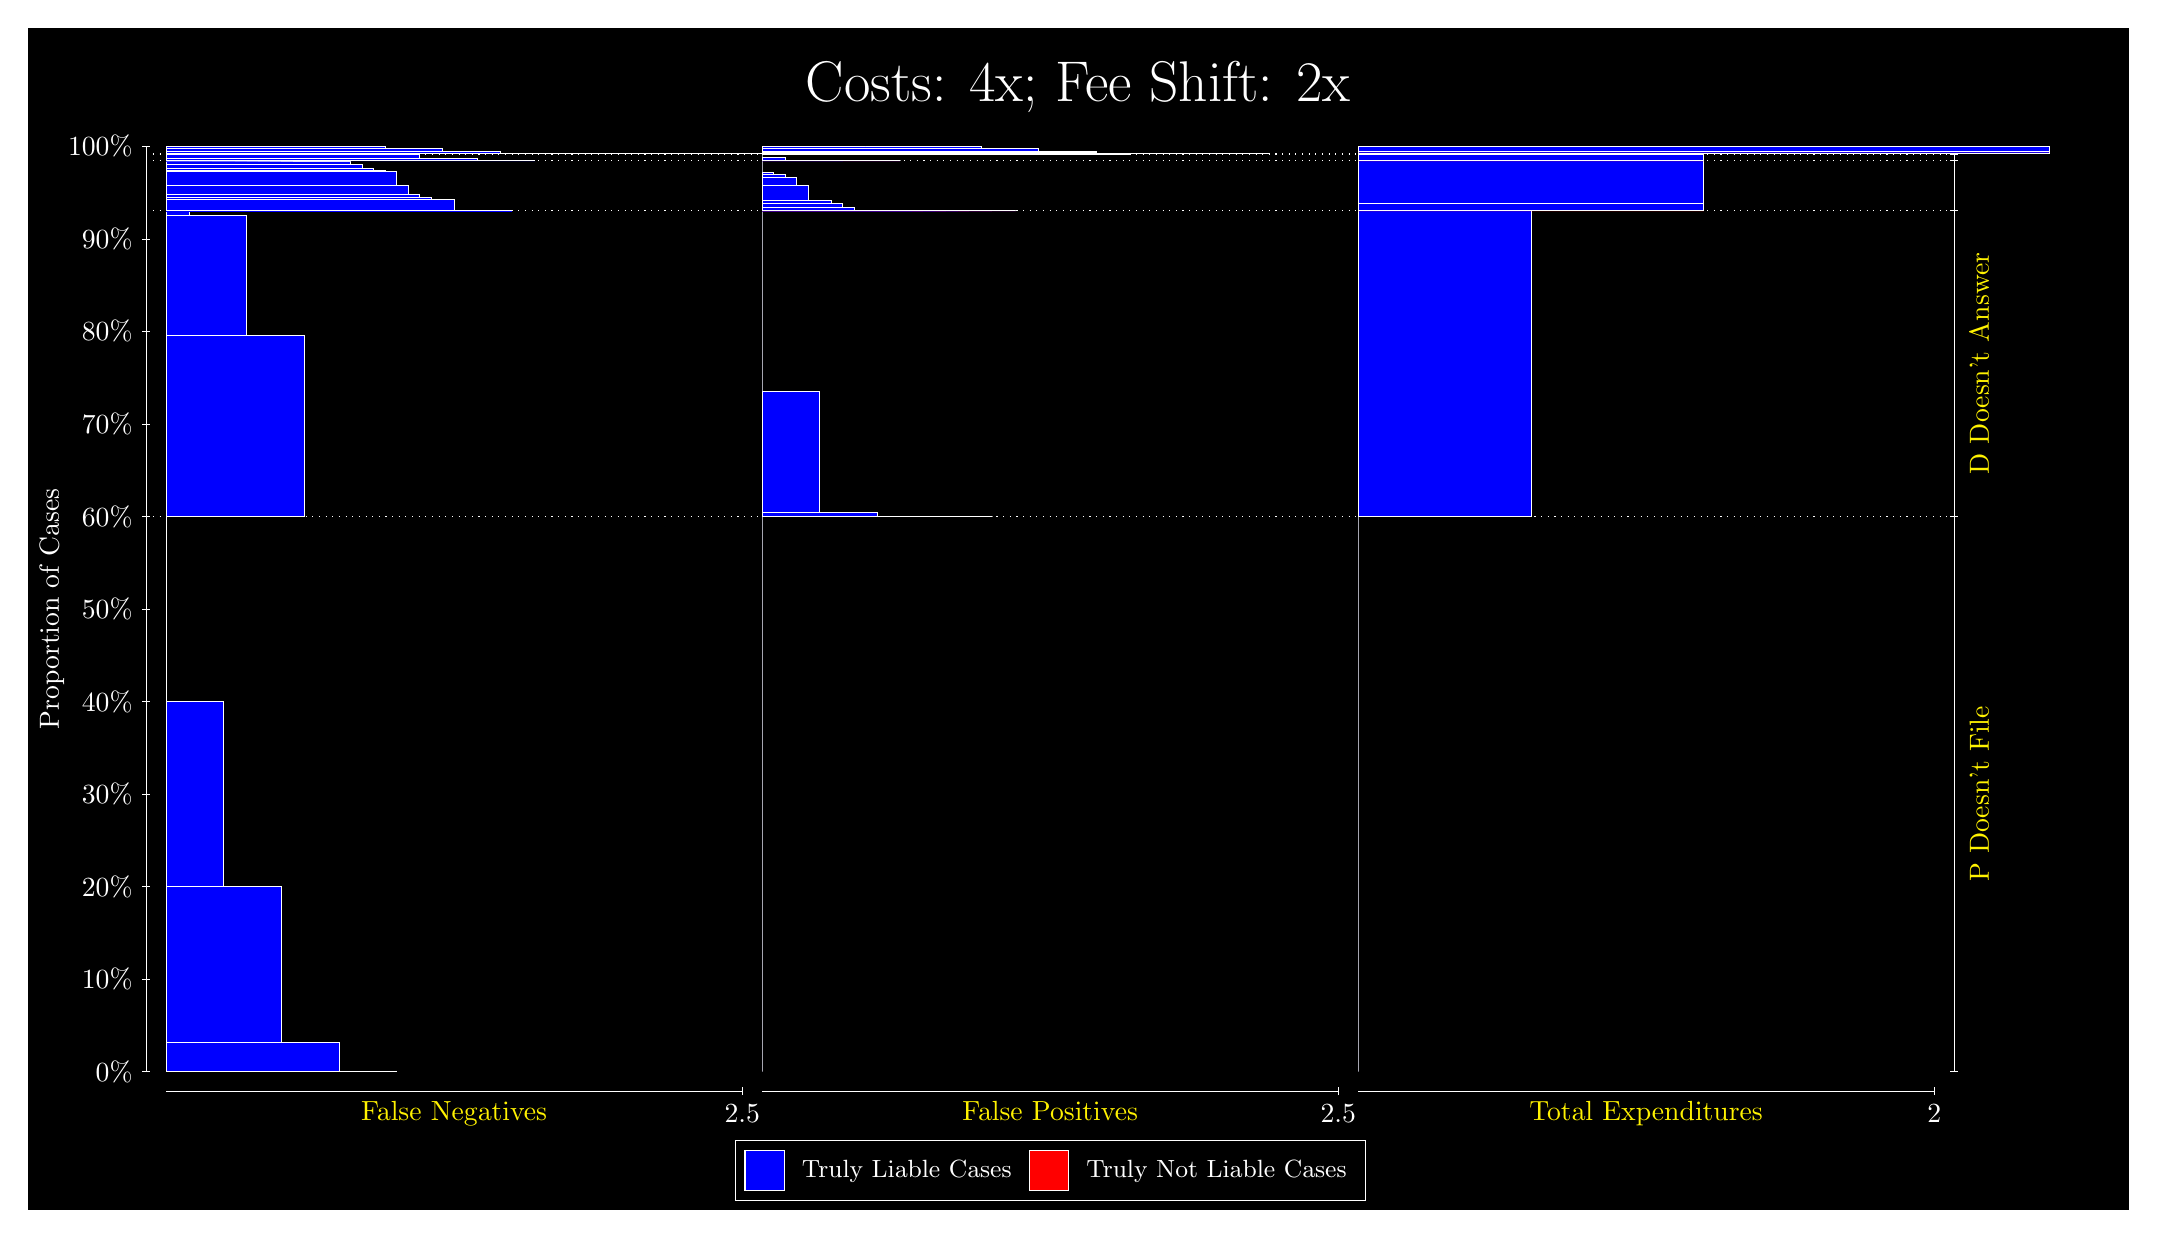
\begin{tikzpicture}
\draw[fill=black] (0,0) rectangle (26.667,15);
\draw[text=white] (0,13.5) rectangle (26.667,15) node[midway] {\huge Costs: 4x; Fee Shift: 2x};
\draw[white, very thin] (1.5,1.75) -- (1.5,13.5);
\node[rotate=90, text=white, anchor=center] at (0.3, 7.625) {Proportion of Cases};
\draw[white, very thin] (1.45,1.75) -- (1.55,1.75);
\node[text=white, anchor=east] at (1.45, 1.75) {0\%};
\draw[white, very thin] (1.45,2.925) -- (1.55,2.925);
\node[text=white, anchor=east] at (1.45, 2.925) {10\%};
\draw[white, very thin] (1.45,4.1) -- (1.55,4.1);
\node[text=white, anchor=east] at (1.45, 4.1) {20\%};
\draw[white, very thin] (1.45,5.275) -- (1.55,5.275);
\node[text=white, anchor=east] at (1.45, 5.275) {30\%};
\draw[white, very thin] (1.45,6.45) -- (1.55,6.45);
\node[text=white, anchor=east] at (1.45, 6.45) {40\%};
\draw[white, very thin] (1.45,7.625) -- (1.55,7.625);
\node[text=white, anchor=east] at (1.45, 7.625) {50\%};
\draw[white, very thin] (1.45,8.8) -- (1.55,8.8);
\node[text=white, anchor=east] at (1.45, 8.8) {60\%};
\draw[white, very thin] (1.45,9.975) -- (1.55,9.975);
\node[text=white, anchor=east] at (1.45, 9.975) {70\%};
\draw[white, very thin] (1.45,11.15) -- (1.55,11.15);
\node[text=white, anchor=east] at (1.45, 11.15) {80\%};
\draw[white, very thin] (1.45,12.325) -- (1.55,12.325);
\node[text=white, anchor=east] at (1.45, 12.325) {90\%};
\draw[white, very thin] (1.45,13.5) -- (1.55,13.5);
\node[text=white, anchor=east] at (1.45, 13.5) {100\%};

\draw[white, very thin] (24.457,1.75) -- (24.457,13.5);
\draw[white, very thin] (24.407,1.75) -- (24.507,1.75);
\node[anchor=west] at (24.407, 1.75) {};
\draw[white, very thin] (24.407,8.8012) -- (24.507,8.8012);
\node[anchor=west] at (24.407, 8.8012) {};
\draw[white, very thin] (24.407,12.682) -- (24.507,12.682);
\node[anchor=west] at (24.407, 12.682) {};
\draw[white, very thin] (24.407,13.317) -- (24.507,13.317);
\node[anchor=west] at (24.407, 13.317) {};
\draw[white, very thin] (24.407,13.401) -- (24.507,13.401);
\node[anchor=west] at (24.407, 13.401) {};
\draw[white, very thin] (24.407,13.414) -- (24.507,13.414);
\node[anchor=west] at (24.407, 13.414) {};
\draw[white, very thin] (24.407,13.5) -- (24.507,13.5);
\node[anchor=west] at (24.407, 13.5) {};

\draw[white, very thin, fill=blue] (1.75,1.75) rectangle (4.6775,1.7538);
\draw[white, very thin, fill=blue] (1.75,1.7538) rectangle (3.9457,2.1271);
\draw[white, very thin, fill=blue] (1.75,2.1271) rectangle (3.2138,4.1043);
\draw[white, very thin, fill=blue] (1.75,4.1043) rectangle (2.4819,6.4512);
\draw[white, very thin, fill=red] (1.75,6.4512) rectangle (1.75,6.4512);
\draw[white, very thin, fill=blue] (1.75,6.4512) rectangle (1.75,8.8012);
\draw[white, very thin, fill=blue] (1.75,8.8012) rectangle (3.5065,11.1);
\draw[white, very thin, fill=blue] (1.75,11.1) rectangle (2.7746,12.629);
\draw[white, very thin, fill=blue] (1.75,12.629) rectangle (2.0428,12.682);
\draw[white, very thin, fill=red] (1.75,12.682) rectangle (1.75,12.682);
\draw[white, very thin, fill=blue] (1.75,12.682) rectangle (1.75,12.682);
\draw[white, very thin, fill=blue] (1.75,12.682) rectangle (6.1413,12.683);
\draw[white, very thin, fill=blue] (1.75,12.683) rectangle (5.8486,12.683);
\draw[white, very thin, fill=blue] (1.75,12.683) rectangle (5.5558,12.689);
\draw[white, very thin, fill=blue] (1.75,12.689) rectangle (5.4094,12.828);
\draw[white, very thin, fill=blue] (1.75,12.828) rectangle (5.2631,12.829);
\draw[white, very thin, fill=blue] (1.75,12.829) rectangle (5.1167,12.857);
\draw[white, very thin, fill=blue] (1.75,12.857) rectangle (4.9703,12.894);
\draw[white, very thin, fill=blue] (1.75,12.894) rectangle (4.8239,13);
\draw[white, very thin, fill=blue] (1.75,13) rectangle (4.6775,13.181);
\draw[white, very thin, fill=blue] (1.75,13.181) rectangle (4.5312,13.19);
\draw[white, very thin, fill=blue] (1.75,13.19) rectangle (4.3848,13.217);
\draw[white, very thin, fill=blue] (1.75,13.217) rectangle (4.2384,13.275);
\draw[white, very thin, fill=blue] (1.75,13.275) rectangle (4.092,13.305);
\draw[white, very thin, fill=blue] (1.75,13.305) rectangle (3.9457,13.308);
\draw[white, very thin, fill=blue] (1.75,13.308) rectangle (3.7993,13.312);
\draw[white, very thin, fill=blue] (1.75,13.312) rectangle (3.6529,13.312);
\draw[white, very thin, fill=blue] (1.75,13.312) rectangle (3.5065,13.317);
\draw[white, very thin, fill=blue] (1.75,13.317) rectangle (3.3602,13.317);
\draw[white, very thin, fill=blue] (1.75,13.317) rectangle (3.2138,13.317);
\draw[white, very thin, fill=blue] (1.75,13.317) rectangle (3.0674,13.317);
\draw[white, very thin, fill=blue] (1.75,13.317) rectangle (2.921,13.317);
\draw[white, very thin, fill=blue] (1.75,13.317) rectangle (2.7746,13.317);
\draw[white, very thin, fill=blue] (1.75,13.317) rectangle (2.6283,13.317);
\draw[white, very thin, fill=blue] (1.75,13.317) rectangle (2.3355,13.317);
\draw[white, very thin, fill=blue] (1.75,13.317) rectangle (2.0428,13.317);
\draw[white, very thin, fill=red] (1.75,13.317) rectangle (1.75,13.317);
\draw[white, very thin, fill=blue] (1.75,13.317) rectangle (6.4341,13.317);
\draw[white, very thin, fill=blue] (1.75,13.317) rectangle (5.7022,13.354);
\draw[white, very thin, fill=blue] (1.75,13.354) rectangle (4.9703,13.401);
\draw[white, very thin, fill=blue] (1.75,13.401) rectangle (4.2384,13.401);
\draw[white, very thin, fill=blue] (1.75,13.401) rectangle (3.5065,13.401);
\draw[white, very thin, fill=red] (1.75,13.401) rectangle (1.75,13.401);
\draw[white, very thin, fill=blue] (1.75,13.401) rectangle (3.5065,13.402);
\draw[white, very thin, fill=blue] (1.75,13.402) rectangle (2.7746,13.411);
\draw[white, very thin, fill=blue] (1.75,13.411) rectangle (2.0428,13.414);
\draw[white, very thin, fill=red] (1.75,13.414) rectangle (1.75,13.414);
\draw[white, very thin, fill=blue] (1.75,13.414) rectangle (1.75,13.414);
\draw[white, very thin, fill=blue] (1.75,13.414) rectangle (15.217,13.414);
\draw[white, very thin, fill=blue] (1.75,13.414) rectangle (14.485,13.414);
\draw[white, very thin, fill=blue] (1.75,13.414) rectangle (13.753,13.415);
\draw[white, very thin, fill=blue] (1.75,13.415) rectangle (13.021,13.415);
\draw[white, very thin, fill=blue] (1.75,13.415) rectangle (12.289,13.415);
\draw[white, very thin, fill=blue] (1.75,13.415) rectangle (11.557,13.415);
\draw[white, very thin, fill=blue] (1.75,13.415) rectangle (10.825,13.415);
\draw[white, very thin, fill=blue] (1.75,13.415) rectangle (7.4587,13.415);
\draw[white, very thin, fill=blue] (1.75,13.415) rectangle (6.7268,13.416);
\draw[white, very thin, fill=blue] (1.75,13.416) rectangle (5.9949,13.436);
\draw[white, very thin, fill=blue] (1.75,13.436) rectangle (5.2631,13.48);
\draw[white, very thin, fill=blue] (1.75,13.48) rectangle (4.5312,13.5);
\draw[white, very thin, fill=blue] (1.75,13.5) rectangle (3.7993,13.5);
\draw[white, very thin, fill=blue] (1.75,13.5) rectangle (3.0674,13.5);
\draw[white, very thin, fill=blue] (1.75,13.5) rectangle (2.3355,13.5);
\draw[white, very thin, fill=red] (1.75,13.5) rectangle (1.75,13.5);
\draw[white, very thin, fill=red] (9.3189,1.75) rectangle (9.3189,1.75);
\draw[white, very thin, fill=blue] (9.3189,1.75) rectangle (9.3189,8.8012);
\draw[white, very thin, fill=red] (9.3189,8.8012) rectangle (12.246,8.8012);
\draw[white, very thin, fill=blue] (9.3189,8.8012) rectangle (12.246,8.8012);
\draw[white, very thin, fill=blue] (9.3189,8.8012) rectangle (11.515,8.8012);
\draw[white, very thin, fill=blue] (9.3189,8.8012) rectangle (10.783,8.8545);
\draw[white, very thin, fill=blue] (9.3189,8.8545) rectangle (10.051,10.383);
\draw[white, very thin, fill=blue] (9.3189,10.383) rectangle (9.3189,12.682);
\draw[white, very thin, fill=red] (9.3189,12.682) rectangle (12.539,12.682);
\draw[white, very thin, fill=blue] (9.3189,12.682) rectangle (12.539,12.682);
\draw[white, very thin, fill=red] (9.3189,12.682) rectangle (12.246,12.682);
\draw[white, very thin, fill=blue] (9.3189,12.682) rectangle (12.246,12.682);
\draw[white, very thin, fill=red] (9.3189,12.682) rectangle (11.954,12.682);
\draw[white, very thin, fill=blue] (9.3189,12.682) rectangle (11.954,12.682);
\draw[white, very thin, fill=blue] (9.3189,12.682) rectangle (11.807,12.682);
\draw[white, very thin, fill=red] (9.3189,12.682) rectangle (11.661,12.682);
\draw[white, very thin, fill=blue] (9.3189,12.682) rectangle (11.661,12.682);
\draw[white, very thin, fill=blue] (9.3189,12.682) rectangle (11.515,12.682);
\draw[white, very thin, fill=red] (9.3189,12.682) rectangle (11.368,12.682);
\draw[white, very thin, fill=blue] (9.3189,12.682) rectangle (11.368,12.682);
\draw[white, very thin, fill=blue] (9.3189,12.682) rectangle (11.222,12.682);
\draw[white, very thin, fill=blue] (9.3189,12.682) rectangle (11.075,12.687);
\draw[white, very thin, fill=blue] (9.3189,12.687) rectangle (10.929,12.687);
\draw[white, very thin, fill=blue] (9.3189,12.687) rectangle (10.783,12.691);
\draw[white, very thin, fill=blue] (9.3189,12.691) rectangle (10.636,12.694);
\draw[white, very thin, fill=blue] (9.3189,12.694) rectangle (10.49,12.724);
\draw[white, very thin, fill=blue] (9.3189,12.724) rectangle (10.344,12.782);
\draw[white, very thin, fill=blue] (9.3189,12.782) rectangle (10.197,12.81);
\draw[white, very thin, fill=blue] (9.3189,12.81) rectangle (10.051,12.818);
\draw[white, very thin, fill=blue] (9.3189,12.818) rectangle (9.9044,12.999);
\draw[white, very thin, fill=blue] (9.3189,12.999) rectangle (9.758,13.106);
\draw[white, very thin, fill=blue] (9.3189,13.106) rectangle (9.6116,13.143);
\draw[white, very thin, fill=blue] (9.3189,13.143) rectangle (9.4652,13.17);
\draw[white, very thin, fill=blue] (9.3189,13.17) rectangle (9.3189,13.317);
\draw[white, very thin, fill=red] (9.3189,13.317) rectangle (11.075,13.317);
\draw[white, very thin, fill=blue] (9.3189,13.317) rectangle (11.075,13.317);
\draw[white, very thin, fill=blue] (9.3189,13.317) rectangle (10.344,13.317);
\draw[white, very thin, fill=blue] (9.3189,13.317) rectangle (9.6116,13.364);
\draw[white, very thin, fill=blue] (9.3189,13.364) rectangle (9.3189,13.401);
\draw[white, very thin, fill=red] (9.3189,13.401) rectangle (14.003,13.401);
\draw[white, very thin, fill=blue] (9.3189,13.401) rectangle (14.003,13.401);
\draw[white, very thin, fill=blue] (9.3189,13.401) rectangle (13.271,13.401);
\draw[white, very thin, fill=blue] (9.3189,13.401) rectangle (12.539,13.404);
\draw[white, very thin, fill=blue] (9.3189,13.404) rectangle (11.807,13.413);
\draw[white, very thin, fill=blue] (9.3189,13.413) rectangle (11.075,13.414);
\draw[white, very thin, fill=red] (9.3189,13.414) rectangle (15.759,13.414);
\draw[white, very thin, fill=blue] (9.3189,13.414) rectangle (15.759,13.414);
\draw[white, very thin, fill=blue] (9.3189,13.414) rectangle (15.028,13.414);
\draw[white, very thin, fill=red] (9.3189,13.414) rectangle (15.028,13.414);
\draw[white, very thin, fill=blue] (9.3189,13.414) rectangle (15.028,13.414);
\draw[white, very thin, fill=blue] (9.3189,13.414) rectangle (14.296,13.414);
\draw[white, very thin, fill=red] (9.3189,13.414) rectangle (14.296,13.414);
\draw[white, very thin, fill=blue] (9.3189,13.414) rectangle (14.296,13.414);
\draw[white, very thin, fill=blue] (9.3189,13.414) rectangle (13.564,13.429);
\draw[white, very thin, fill=red] (9.3189,13.429) rectangle (13.564,13.429);
\draw[white, very thin, fill=blue] (9.3189,13.429) rectangle (13.564,13.434);
\draw[white, very thin, fill=blue] (9.3189,13.434) rectangle (12.832,13.436);
\draw[white, very thin, fill=blue] (9.3189,13.436) rectangle (12.832,13.478);
\draw[white, very thin, fill=blue] (9.3189,13.478) rectangle (12.1,13.498);
\draw[white, very thin, fill=blue] (9.3189,13.498) rectangle (11.368,13.499);
\draw[white, very thin, fill=blue] (9.3189,13.499) rectangle (10.636,13.499);
\draw[white, very thin, fill=red] (9.3189,13.499) rectangle (9.3189,13.499);
\draw[white, very thin, fill=blue] (9.3189,13.499) rectangle (9.3189,13.5);
\draw[white, very thin, fill=red] (16.888,1.75) rectangle (16.888,1.75);
\draw[white, very thin, fill=blue] (16.888,1.75) rectangle (16.888,8.8012);
\draw[white, very thin, fill=red] (16.888,8.8012) rectangle (19.083,8.8012);
\draw[white, very thin, fill=blue] (16.888,8.8012) rectangle (19.083,12.682);
\draw[white, very thin, fill=red] (16.888,12.682) rectangle (21.279,12.682);
\draw[white, very thin, fill=blue] (16.888,12.682) rectangle (21.279,12.782);
\draw[white, very thin, fill=red] (16.888,12.782) rectangle (21.279,12.782);
\draw[white, very thin, fill=blue] (16.888,12.782) rectangle (21.279,13.317);
\draw[white, very thin, fill=red] (16.888,13.317) rectangle (21.279,13.317);
\draw[white, very thin, fill=blue] (16.888,13.317) rectangle (21.279,13.401);
\draw[white, very thin, fill=red] (16.888,13.401) rectangle (21.279,13.401);
\draw[white, very thin, fill=blue] (16.888,13.401) rectangle (21.279,13.414);
\draw[white, very thin, fill=red] (16.888,13.414) rectangle (25.67,13.414);
\draw[white, very thin, fill=blue] (16.888,13.414) rectangle (25.67,13.431);
\draw[white, very thin, fill=red] (16.888,13.431) rectangle (25.67,13.431);
\draw[white, very thin, fill=blue] (16.888,13.431) rectangle (25.67,13.499);
\draw[white, very thin, fill=red] (16.888,13.499) rectangle (25.67,13.499);
\draw[white, very thin, fill=blue] (16.888,13.499) rectangle (25.67,13.5);
\draw[white, dotted] (1.5,8.8012) -- (24.457,8.8012);
\draw[white, dotted] (1.5,12.682) -- (24.457,12.682);
\draw[white, dotted] (1.5,13.317) -- (24.457,13.317);
\draw[white, dotted] (1.5,13.401) -- (24.457,13.401);
\draw[white, dotted] (1.5,13.414) -- (24.457,13.414);
\draw[white, very thin] (1.75,1.5) -- (9.0689,1.5);
\node[text=yellow, anchor=north] at (5.4094, 1.5) {False Negatives};
\draw[white, very thin] (9.0689,1.45) -- (9.0689,1.55);
\node[text=white, anchor=north] at (9.0689, 1.45) {2.5};

\draw[white, very thin] (9.3189,1.5) -- (16.638,1.5);
\node[text=yellow, anchor=north] at (12.978, 1.5) {False Positives};
\draw[white, very thin] (16.638,1.45) -- (16.638,1.55);
\node[text=white, anchor=north] at (16.638, 1.45) {2.5};

\draw[white, very thin] (16.888,1.5) -- (24.207,1.5);
\node[text=yellow, anchor=north] at (20.547, 1.5) {Total Expenditures};
\draw[white, very thin] (24.207,1.45) -- (24.207,1.55);
\node[text=white, anchor=north] at (24.207, 1.45) {2};

\node[text=yellow, centered, rotate=90] at (24.777, 5.2756) {P Doesn't File};
\node[text=yellow, centered, rotate=90] at (24.777, 10.742) {D Doesn't Answer};





\draw (12.978300999999998,1.5) node[draw=none] (baseCoordinate) {};
\begin{scope}[align=center]
        \matrix[scale=0.5, draw=white, below=0.5cm of baseCoordinate, nodes={draw}, column sep=0.1cm]{
            \node[rectangle, draw, minimum width=0.5cm, minimum height=0.5cm, fill=blue] {}; &
            \node[draw=none, font=\small, text=white] (B) {Truly Liable Cases}; &
            \node[rectangle, draw, minimum width=0.5cm, minimum height=0.5cm, fill=red] {}; &
            \node[draw=none, font=\small, text=white] (B) {Truly Not Liable Cases}; \\
            };
\end{scope}

\end{tikzpicture}
\end{document}